\chapter{Trigonométrie}

\section{Cercle trigonométrique et radian}

\subsection{Le cercle trigonométrique}

\begin{defin}
	Sur un cercle, on appelle \textbf{sens direct}, \textbf{sens positif} ou \textbf{sens trigonométrique} le sens contraire des aiguilles d'une montre.

	Le sens des aiguilles d'une montre est appelé \textbf{sens indirect}.
\end{defin}

\begin{defin}
	Dans le plan muni d'un repère orthonormé $\vOIJ$ orienté dans le sens direct, le \textbf{cercle trigonométrique} est le cercle de centre $O$ et de rayon $1$.

	\begin{center}
		\begin{tikzpicture}[scale=1.5]
			\draw[->] (-1.2,0) -- (1.5,0) node[above] {$x$};
			\draw[->] (0,-1.2) -- (0,1.5) node[right] {$y$};
			\draw[bleu] (0,0) circle (1);
			\filldraw (0,0) circle (1pt);
			\filldraw (1,0) circle (1pt) node[below right] {$I$};
			\filldraw (0,1) circle (1pt) node[above left] {$J$};
			\node[below left] at (0,0) {$O$};
			\draw[rouge, ultra thick, -{Stealth[length=3mm]}] (0.94,0.34) arc[start angle=20, end angle=70, radius=1];
			\node[rouge, right] at (0.7,0.85) {sens direct};
		\end{tikzpicture}
	\end{center}
\end{defin}

\subsection{Le radian}

\begin{prop}
	La longueur du cercle trigonométrique est égale à $2\pi$.
\end{prop}

\begin{demo}
	Son rayon vaut $1$, donc $P = 2\pi R = 2\pi \times 1 = 2\pi$.
\end{demo}

\begin{defin}
	Ainsi, à un tour complet sur le cercle, on peut faire correspondre le nombre réel $2\pi$.

	On définit alors une nouvelle unité d'angle : le \textbf{radian}, tel qu'un tour complet mesure $360\,\degres$ ou $2\pi$ radians.

	\begin{center}
		\begin{tikzpicture}[scale=1.8, >=Stealth]
			\draw[gris, thin, ->] (-1.5,0) -- (1.7,0) node[right] {$x$};
			\draw[gris, thin, ->] (0,-1.5) -- (0,1.6) node[above] {$y$};
			\draw[violet, dashed, -{Stealth[length=3mm]}] (5:1.28) arc[start angle=5, end angle=355, radius=1.28];
			\node[violet, rotate=90, fill=white] at (-1.55,-0.1) {$1$ tour $=2\pi$};
			\draw[bleu, thick] (0,0) circle (1);
			\coordinate (M) at (50:1);
			\draw[rouge, thick] (0,0) -- (1,0);
			\draw[rouge, thick] (0,0) -- (M);
			\draw[rouge, ultra thick, -{Stealth[length=2.5mm]}] (1,0) arc[start angle=0, end angle=50, radius=1];
			\draw[rouge, thick] (0.45,0) arc[start angle=0, end angle=50, radius=0.45];
			\node[rouge] at (25:0.62) {$\alpha$};
			\node[rouge, rotate=25, right, fill=white] at (25:1.08) {arc $= \alpha$};
			\fill (0,0) circle (1pt) node[below left] {$O$};
			\fill[bleu] (1,0) circle (1pt) node[below right] {$I$};
			\fill[bleu] (0,1) circle (1pt) node[above left] {$J$};
			\node[above right, fill=white] at (M) {$M$};
			\fill[rouge] (M) circle (1pt);
		\end{tikzpicture}
	\end{center}

\end{defin}

\begin{rem}
	La longueur d'un quart de cercle trigonométrique est $\frac{\pi}{2}$.
\end{rem}

\subsection{Correspondance degrés et radians}

Puisqu'à $2\pi$ radians on fait correspondre un angle de $360\,\degres$, la mesure en radians est proportionnelle à la mesure en degrés. On obtient les correspondances suivantes :

\begin{center}
	\rnc{\arraystretch}{1.6}
	\begin{tabular}{|c|c|c|c|c|c|c|c|c|} \hline
		\ccg Angle en degrés                       & $0\,\degres$ & $30\,\degres$    & $45\,\degres$    & $60\,\degres$    & $90\,\degres$    & $180\,\degres$ & $270\,\degres$    & $360\,\degres$ \\ \hline
		\rule[-4mm]{0mm}{11mm}\ccg Angle en radian & $0$          & $\dfrac{\pi}{6}$ & $\dfrac{\pi}{4}$ & $\dfrac{\pi}{3}$ & $\dfrac{\pi}{2}$ & $\pi$          & $\dfrac{3\pi}{2}$ & $2\pi$         \\ \hline
	\end{tabular}

	\rule{0mm}{1mm}

	\begin{tikzpicture}[scale=3]
		\tikzstyle{axes}=[thin, gris, ->]
		\tikzstyle{cercle}=[thick, blue!70!black]
		\tikzstyle{angle_deg}=[fill=white, inner sep=1pt]
		\tikzstyle{angle_rad}=[rouge]
		\def\r{1.1}
		\draw[cercle] (0, 0) circle (\r);
		\foreach \deg/\rad in {
		0/{0}, 30/{\frac{\pi}{6}}, 45/{\frac{\pi}{4}}, 60/{\frac{\pi}{3}}, 90/{\frac{\pi}{2}}, 120/{\frac{2\pi}{3}}, 135/{\frac{3\pi}{4}}, 150/{\frac{5\pi}{6}}, 180/{\pi}, 210/{\frac{7\pi}{6}}, 225/{\frac{5\pi}{4}}, 240/{\frac{4\pi}{3}}, 270/{\frac{3\pi}{2}}, 300/{\frac{5\pi}{3}}, 315/{\frac{7\pi}{4}}, 330/{\frac{11\pi}{6}}
		}
		{
		\draw[thin, lightgray] (0, 0) -- (\deg:\r);
		\node[angle_deg] at (\deg:\r*1.15) {\ang{\deg}};
		\node[angle_rad, fill=white] at (\deg:\r*0.8) {$\rad$};
		\filldraw (\deg:\r) circle (0.5pt);
		}
		\filldraw (0,0) circle (0.5pt);
		\node[below left] at (0, 0) {$O$};
	\end{tikzpicture}
\end{center}

\begin{methode}[Passer des degrés aux radians et réciproquement]
	Pour convertir une mesure d'angle :

	\begin{center}
		\begin{tikzpicture}[node distance=3.5cm, auto, thick, >=Stealth]
			\node[draw, rectangle, minimum width=2.5cm, minimum height=1cm, rounded corners, fill=gray!10, align=center] (deg) {\textbf{Degrés}};
			\node[draw, rectangle, minimum width=2.5cm, minimum height=1cm, rounded corners, fill=gray!10, align=center, right=of deg] (rad) {\textbf{Radians}};
			\draw[->, thick] ([yshift=3mm]deg.east) -- node[above] {$\times \dfrac{\pi}{180}$} ([yshift=3mm]rad.west);
			\draw[<-, thick] ([yshift=-3mm]deg.east) -- node[below] {$\times \dfrac{180}{\pi}$} ([yshift=-3mm]rad.west);
		\end{tikzpicture}
	\end{center}

	\begin{enumerate}
		\item Donner la mesure en radians de l'angle de mesure $33\,\degres$.
		\item Donner la mesure en degrés de l'angle de mesure $\dfrac{3\pi}{8}$ radians.
	\end{enumerate}

	\begin{correction}
		\nline
		\begin{multicols}{2}
			\begin{enumerate}
				\item $33 \times \dfrac{\pi}{180} = \dfrac{33\pi}{180} = \dfrac{11\pi}{60}$
				\item $\dfrac{3\pi}{8} \times \dfrac{180}{\pi} = 67{,}5\,\degres$
			\end{enumerate}
		\end{multicols}
	\end{correction}
\end{methode}

\newpage

\section{Mesure d'un angle orienté}

\subsection{Lire sur le cercle trigonométrique}

\begin{rem}
	\nline
	\begin{wrapstuff}[r]
		\begin{tikzpicture}[scale=1.7, >=stealth]
			\draw[gris, thin, ->] (-1.4,0) -- (1.4,0) node[below] {$x$};
			\draw[gris, thin, ->] (0,-1.4) -- (0,1.4) node[left] {$y$};
			\draw[black] (0,0) circle (1);
			\draw[very thick, rouge] (1,0) arc[start angle=0, end angle=85, radius=1];
			\draw[very thick, bleu] (0.86,0) arc[start angle=0, end angle=-267, radius=0.86];
			\draw[very thick, violet] (1.14,0) arc[start angle=0, end angle=450, radius=1.14];
			\draw[very thick, ->, rouge] ({cos(80)},{sin(80)}) arc[start angle=80, end angle=88, radius=1];
			\draw[very thick, ->, bleu] ({0.86*cos{-260}},{0.86*sin{-260}}) arc[start angle=-260, end angle=-270, radius=0.86];
			\draw[very thick, ->, violet] ({1.14*cos(80)},{1.14*sin(80)}) arc[start angle=80, end angle=89, radius=1.14];
			\node[rouge] at (52:0.78) {$\frac{\pi}{2}$};
			\node[bleu] at (200:0.66) {$\frac{-3\pi}{2}$};
			\node[violet] at (300:1.34) {$\frac{5\pi}{2}$};
			\fill (0,0) circle (1pt) node[below left] {$O$};
			\fill[gris!60] (1,0) circle (1pt);
			\fill[rouge] (0,1) circle (1pt);
		\end{tikzpicture}
	\end{wrapstuff}

	Un point du cercle trigonométrique peut être associé à \textbf{plusieurs} nombres réels.

	Le point associé à l'angle droit peut être repéré par $\dfrac{\pi}{2}$ (lecture dans le sens direct), mais aussi par $\dfrac{-3\pi}{2}$ (lecture dans le sens indirect) ou encore par $\dfrac{5\pi}{2}$ (un tour supplémentaire dans le sens direct).

	Les mesures $\dfrac{\pi}{2}$, $\dfrac{-3\pi}{2}$ et $\dfrac{5\pi}{2}$ sont donc associées à un même point du cercle.

	\rule{0mm}{8mm}
\end{rem}

\begin{methode}[Lire sur le cercle trigonométrique le nombre associé à un point]
	\nline
	\begin{wrapstuff}[r]
		\begin{tikzpicture}[scale=1.5, >=Stealth]
			\draw[gris, thin, ->] (-1.2,0) -- (1.4,0) node[above] {$x$};
			\draw[gris, thin, ->] (0,-1.2) -- (0,1.4) node[right] {$y$};
			\foreach \a in {45,135,...,315} \draw[gray, dashed, thin] (\a:0) -- (\a:1);
			\draw[bleu, very thick] (0,0) circle (1);
			\fill[gris] (45:1) circle (1pt) node[above right] {$\frac{\pi}{4}$};
			\coordinate (A) at (225:1);
			\draw[rouge, thick] (0,0) -- (A);
			\fill[rouge] (A) circle (1.5pt) node[below left] {$A$};
			\node[above right, fill=white] (0,0) {$O$};
			\fill (0,0) circle (1.5pt);
			\fill[gris] (1,0) circle (1.5pt) node[below right] {$I$};
			\fill[gris] (0,1) circle (1.5pt) node[above left] {$J$};
		\end{tikzpicture}
	\end{wrapstuff}

	Un même point du cercle trigonométrique est associé à une infinité de nombres réels, qui se déduisent les uns des autres en ajoutant ou retranchant des tours complets ($2\pi$).

	Pour lire le nombre associé à un point, on précise l'intervalle dans lequel on cherche.

	On considère le point $A$ représenté ci-dessus.

	\begin{enumerate}
		\item Donner une mesure de l'angle associé à $A$ sur $\intff{0}{2\pi}$.
		\item Donner une mesure de l'angle associé à $A$ sur $\intff{-\pi}{\pi}$.
	\end{enumerate}

	\phantom{x}

	\begin{correction}
		On a :

		\begin{enumerate}
			\item \textbf{Sur $\intff{0}{2\pi}$.}

			      En partant de $I$ et en tournant dans le sens direct, on compte $5 \times \dfrac{\pi}{4}$ pour atteindre $A$.

			      Le point $A$ est donc associé à $\dfrac{5\pi}{4}$, qui appartient bien à $\intff{0}{2\pi}$.

			\item \textbf{Sur $\intff{-\pi}{\pi}$.}

			      En partant de $I$ et en tournant dans le sens indirect, on compte $3 \times \left(\dfrac{-\pi}{4}\right)$ pour atteindre $A$.

			      Le point $A$ est donc associé à $\dfrac{-3\pi}{4}$, qui appartient bien à $\intff{-\pi}{\pi}$.
		\end{enumerate}
	\end{correction}
\end{methode}

\begin{rem}
	Le point $A$ est associé à $\dfrac{5\pi}{4}$, mais aussi à :

	\begin{multicols}{2}
		\begin{itemize}
			\item $\dfrac{5\pi}{4} - 2\pi = \dfrac{-3\pi}{4}\quad$ (moins un tour)
			\item $\dfrac{5\pi}{4} + 2\pi = \dfrac{13\pi}{4}\quad$ (plus un tour)
			\item $\dfrac{5\pi}{4} - 4\pi = \dfrac{-11\pi}{4}\quad$ (moins deux tours)
			\item \dots
		\end{itemize}
	\end{multicols}

	Plus généralement, $A$ est associé à \textbf{tous les nombres de la forme} $\dfrac{5\pi}{4} + 2k\pi$, où $k$ est un entier relatif.
\end{rem}

\newpage

\begin{methode}[Placer un point sur le cercle trigonométrique]
	Placer sur le cercle trigonométrique le point associé au nombre $\dfrac{9\pi}{4}$.

	\begin{correction}
		On fait apparaître un tour complet ($2\pi$) :
		\[
			\dfrac{9\pi}{4} = \dfrac{8\pi}{4} + \dfrac{\pi}{4} = 2\pi + \dfrac{\pi}{4}.
		\]

		$\dfrac{9\pi}{4}$ correspond donc à un tour complet dans le sens direct suivi de $\dfrac{\pi}{4}$.

		Le point a la même position sur le cercle que le point associé à $\dfrac{\pi}{4}$.

		\begin{center}
			\begin{tikzpicture}[scale=1.5, >=Stealth]
				\draw[gris, thin, ->] (-1.2,0) -- (1.4,0) node[above] {$x$};
				\draw[gris, thin, ->] (0,-1.2) -- (0,1.4) node[right] {$y$};
				\foreach \a in {45,135,...,315} \draw[gray, dashed, thin] (\a:0) -- (\a:1);
				\draw[bleu, very thick] (0,0) circle (1);
				\draw[violet, ->, thick] (1,0) arc[start angle=0, end angle=403, radius=1];
				\draw[rouge, thick] (0,0) -- (45:1);
				\fill[rouge] (45:1) circle (1.5pt) node[above right] {$M$};
				\node[above right, fill=white] (0,0) {$O$};
				\fill (0,0) circle (1.5pt);
				\fill[gris] (1,0) circle (1.5pt) node[below right] {$I$};
				\fill[gris] (0,1) circle (1.5pt) node[above left] {$J$};
			\end{tikzpicture}
		\end{center}
	\end{correction}
\end{methode}

\begin{methode}[Placer un point sur le cercle trigonométrique (grande mesure)]
	Placer sur le cercle trigonométrique le point associé au nombre $\dfrac{193\pi}{6}$.

	\begin{correction}
		On cherche combien de tours complets ($2\pi$) contient $\dfrac{193\pi}{6}$.

		On effectue la division euclidienne de $193$ par $6$ :
		\[
			\begin{array}{r|l}
				193            & 6  \\
				\cline{2-2}
				-18\phantom{x} & 32 \\
				\phantom{x}13  &    \\
				-12            &    \\
				\phantom{xx}1  &    \\
			\end{array}
			\qquad\implies 193 = 6 \times 32 + 1
		\]

		On en déduit :
		\[
			\def\arraystretch{2}
			\begin{array}{rcl}
				\dfrac{193\pi}{6} & = & \dfrac{(6 \times 32 + 1)\pi}{6}                                                                                     \\
				                  & = & \dfrac{(6 \times 32)\pi}{6} + \dfrac{1\pi}{6} \quad =32\pi + \dfrac{\pi}{6} \quad = 16 \times 2\pi + \dfrac{\pi}{6}
			\end{array}
		\]

		$\dfrac{193\pi}{6}$ correspond donc à $16$ tours complets dans le sens direct suivis de $\dfrac{\pi}{6}$.

		Le point a la même position sur le cercle que le point associé à $\dfrac{\pi}{6}$.

		\begin{center}
			\begin{tikzpicture}[scale=1.5, >=Stealth]
				\draw[gris, thin, ->] (-1.2,0) -- (1.4,0) node[above] {$x$};
				\draw[gris, thin, ->] (0,-1.2) -- (0,1.4) node[right] {$y$};
				\foreach \a in {30,60,...,330} \draw[gray, dashed, thin] (\a:0) -- (\a:1);
				\draw[bleu, very thick] (0,0) circle (1);
				\draw[violet, ->, thick] (1,0) arc[start angle=0, end angle=390, radius=1];
				\node[violet, right, font=\small] at (-50:1.18) {$16$ tours $+\ \frac{\pi}{6}$};
				\draw[rouge, thick] (0,0) -- (30:1);
				\fill[rouge] (30:1) circle (1.5pt) node[above right] {$M$};
				\node[above right, fill=white] (0,0) {$O$};
				\fill (0,0) circle (1.5pt);
				\fill[gris] (1,0) circle (1.5pt) node[below right] {$I$};
				\fill[gris] (0,1) circle (1.5pt) node[above left] {$J$};
			\end{tikzpicture}
		\end{center}
	\end{correction}
\end{methode}

\subsection{Mesure principale d'un angle orienté}

\begin{defin}
	Soit $\vec{u}$ et $\vec{v}$ deux vecteurs non nuls du plan.

	Il existe une unique mesure de l'angle orienté $\pa{\vec{u}\,,\,\vec{v}}$ appartenant à l'intervalle $\intof{-\pi}{\pi}$ : cette mesure est appelée \textbf{mesure principale} de l'angle $\pa{\vec{u}\,,\,\vec{v}}$.

	\begin{center}
		\begin{tikzpicture}[scale=2, >=Stealth]
			\draw[gris, thin, ->] (-1.3,0) -- (1.5,0) node[above] {$x$};
			\draw[gris, thin, ->] (0,-1.3) -- (0,1.5) node[right] {$y$};
			\draw[bleu, dotted, thick] (0,0) circle (1);
			\coordinate (U) at (20:1);
			\coordinate (V) at (130:1);
			\draw[rouge, thick, ->] (0,0) -- (U) node[midway, sloped, above] {$\vec{u}$};
			\draw[vert, thick, ->] (0,0) -- (V) node[midway, sloped, above] {$\vec{v}$};
			\coordinate (Ap) at (20:1);
			\coordinate (Bp) at (130:1);
			\draw[orange, very thick, ->] (20:1) arc[start angle=20, end angle=130, radius=1];
			\node[below left, fill=white] (0,0) {$O$};
			\fill (0,0) circle (1.3pt);
			\node[orange] at (60:1.125) {$\alpha$};
			\fill[rouge] (Ap) circle (1.3pt) node[right] {$A'$};
			\fill[vert] (Bp) circle (1.3pt) node[left] {$B'$};
		\end{tikzpicture}
	\end{center}

\end{defin}

\begin{rem}
	Cette mesure correspond au trajet le plus court de $A'$ à $B'$ sur le cercle.
\end{rem}

\begin{methode}[Donner la mesure principale d'un angle]
	Donner la mesure principale de l'angle $\dfrac{27\pi}{4}$.

	\begin{correction}
		\nline
		\begin{itemize}
			\item On choisit un multiple de $4$ proche de $27$, soit $28$ :
			      \[
				      \dfrac{27\pi}{4} = \dfrac{28\pi}{4} - \dfrac{\pi}{4} \quad = 7\pi - \dfrac{\pi}{4}.
			      \]
			\item Dans $7\pi$, on fait apparaître un multiple de $2\pi$, soit $6\pi$ :
			      \[
				      \dfrac{27\pi}{4} = 6\pi + \pi - \dfrac{\pi}{4} \quad = 6\pi + \dfrac{4\pi}{4} - \dfrac{\pi}{4} \quad = 6\pi + \dfrac{3\pi}{4}.
			      \]
			\item $6\pi$ correspond à $3$ tours entiers, et $\dfrac{3\pi}{4}$ est bien compris dans $\intof{-\pi}{\pi}$.
		\end{itemize}

		La mesure principale de $\dfrac{27\pi}{4}$ est donc $\dfrac{3\pi}{4}$.
	\end{correction}
\end{methode}

\newpage

\section{Sinus et cosinus}

\subsection{Définitions et propriétés}

On considère un angle orienté $\pa{\vec{u}\,,\,\vec{v}}$ dont $\alpha$ est une mesure en radians, et on appelle $M$ le point du cercle trigonométrique associé à $\alpha$.

\begin{defin}
	Soit $M$ le point du cercle trigonométrique associé au nombre $x$.
	\begin{itemize}
		\item Le \textbf{cosinus} de $x$ est \textbf{l'abscisse} de $M$ ; on note $\cos(x)$.
		\item Le \textbf{sinus} de $x$ est \textbf{l'ordonnée} de $M$ ; on note $\sin(x)$.
	\end{itemize}
\end{defin}

\begin{center}
	\begin{tikzpicture}[scale=2.3]
		\draw[->] (-1.2,0) -- (1.3,0) node[above] {$x$};
		\draw[->] (0,-1.2) -- (0,1.3) node[right] {$y$};
		\coordinate (M) at (50:1);
		\draw[rouge, thick] (0,0) -- (M);
		\draw[bleu, dashed] (M) -- (M |- 0,0) node[below, fill=white, font=\small] {$\cos(x)$};
		\draw[bleu, dashed] (M) -- (M -| 0,0) node[left, fill=white, font=\small] {$\sin(x)$};
		\draw[orange, thick] (0.5,0) arc[start angle=0, end angle=50, radius=0.5] node[midway, fill=white] {$x$};
		\draw[bleu, thick] (0,0) circle (1);
		\node[above right, fill=white, font=\small] at (M |- 0,0) {$H$};
		\fill[rouge] (M) circle (1pt) node[above right] {$M$};
		\fill[bleu] (M |- 0,0) circle (1pt);
		\fill[bleu] (M -| 0,0) circle (1pt);
		\fill (0,0) circle (1pt) node[below left] {$O$};
	\end{tikzpicture}
\end{center}

\begin{prop}
	Pour tout réel $x$, on a :
	\begin{enumerate}
		\item $-1 \leqslant \sin(x) \leqslant 1\ $ et $\ -1 \leqslant \cos(x) \leqslant 1$ \hfill (propriété d'encadrement)
		\item $\cos^2(x) + \sin^2(x) = 1$ \hfill (propriété fondamentale)
	\end{enumerate}
\end{prop}

\begin{demo}
	\nline
	\begin{enumerate}
		\item Le cercle trigonométrique est de rayon $1$, donc les coordonnées de $M$ sont comprises entre $-1$ et $1$ :
		      \begin{itemize}
			      \item $-1 \leqslant \sin(x) \leqslant 1$
			      \item $-1 \leqslant \cos(x) \leqslant 1$.
		      \end{itemize}
		\item Dans le triangle $OHM$ rectangle en $H$, le théorème de Pythagore permet d'établir que :
		      \[
			      \begin{array}{rccccl}
				           & OH^2              & + & HM^2              & = & OM^2 \\
				      \iff & \pa{\cos\pa{x}}^2 & + & \pa{\sin\pa{x}}^2 & = & 1    \\
				      \iff & \cos^2 \pa{x}     & + & \sin^2 \pa{x}     & = & 1
			      \end{array}
		      \]
	\end{enumerate}
\end{demo}

\subsection{Valeurs remarquables}

\begin{prop}
	\nline
	\begin{center}
		\rnc{\arraystretch}{2}
		\begin{tabular}{|c|c|c|c|c|c|c|} \hline
			\rule[-4mm]{0mm}{11mm}\ccg $x$       & $0$ & $\dfrac{\pi}{6}$      & $\dfrac{\pi}{4}$      & $\dfrac{\pi}{3}$      & $\dfrac{\pi}{2}$ & $\pi$ \\ \hline
			\rule[-4mm]{0mm}{11mm}\ccg $\cos(x)$ & $1$ & $\dfrac{\sqrt{3}}{2}$ & $\dfrac{\sqrt{2}}{2}$ & $\dfrac{1}{2}$        & $0$              & $-1$  \\ \hline
			\rule[-4mm]{0mm}{11mm}\ccg $\sin(x)$ & $0$ & $\dfrac{1}{2}$        & $\dfrac{\sqrt{2}}{2}$ & $\dfrac{\sqrt{3}}{2}$ & $1$              & $0$   \\ \hline
		\end{tabular}
	\end{center}
\end{prop}

\begin{rem}
	Pour tout $\alpha \neq \dfrac{\pi}{2}$, on définit la tangente par $\tan(\alpha) = \dfrac{\sin(\alpha)}{\cos(\alpha)}$.
\end{rem}

\begin{demo}
	\nline
	\begin{itemize}
		\item Les points associés à $0$, $\dfrac{\pi}{2}$ et $\pi$ sont respectivement $I\coordl{1}{0}$, $J\coordl{0}{1}$ et le point de coordonnées $\coordl{-1}{0}$ donc :
		      \begin{center}
			      \rnc{\arraystretch}{1.2}
			      \begin{tabular}{|c|c|c|c|} \hline
				      \ccg $x$       & $0$ & $\frac{\pi}{2}$ & $\pi$ \\ \hline
				      \ccg $\cos(x)$ & $1$ & $0$             & $-1$  \\ \hline
				      \ccg $\sin(x)$ & $0$ & $1$             & $0$   \\ \hline
			      \end{tabular}
		      \end{center}

		\item Soit $M$ le point associé à $\dfrac{\pi}{4}$ (soit $45^\circ$). Il est situé sur la bissectrice de l'angle $\widehat{IOJ}$ : son abscisse et son ordonnée sont égales et positives, notons-les $a$.

		      Comme $\cos^2 x + \sin^2 x = 1$, on a $2a^2 = 1$, donc $a = \sqrt{\dfrac{1}{2}} = \dfrac{\sqrt{1} \times \sqrt{2} }{\sqrt{2} \times \sqrt{2}} = \dfrac{\sqrt{2}}{2}$.

		      \begin{center}
			      \begin{tikzpicture}[scale=3, font=\footnotesize]
				      \clip (-0.4,-0.3) rectangle (1.35,1.35);
				      \draw[->, thick] (-0.2,0) -- (1.3,0) node[above] {$x$};
				      \draw[->, thick] (0,-0.2) -- (0,1.3) node[right] {$y$};
				      \node[below left] at (0,0) {$O$};
				      \fill (1,0) circle (0.6pt) node[below right] {$1$};
				      \fill (0,1) circle (0.6pt) node[above left] {$1$};
				      \draw[thick] (0,0) circle (1);
				      \draw[gray, dashed] (0,0) -- (0.71,0.71);
				      \coordinate (M) at ({cos(45)}, {sin(45)});
				      \node[above right, red] at (M) {$M\left(\dfrac{\sqrt{2}}{2}, \dfrac{\sqrt{2}}{2}\right)$};
				      \draw[dashed, blue] (M) -- ({cos(45)}, 0) node[below, black] {$a = \dfrac{\sqrt{2}}{2}$};
				      \draw[dashed, blue] (M) -- (0, {sin(45)}) node[left, black] {$a = \dfrac{\sqrt{2}}{2}$};
				      \draw (0.3,0) arc (0:45:0.3);
				      \node at (0.38, 0.16) {$\dfrac{\pi}{4}$};
				      \fill[red] (M) circle (0.6pt);
			      \end{tikzpicture}
			      $\qquad\implies\qquad\cos{\dfrac{\pi}{4}} = \dfrac{\sqrt{2}}{2}\ $ et $\ \sin{\dfrac{\pi}{4}}=\dfrac{\sqrt{2}}{2}$
		      \end{center}

		\item Soit $M$ le point associé à $\dfrac{\pi}{3}$ (soit $60^\circ$). Le triangle $OIM$ est isocèle en $O$ et son angle en $O$ mesure $60^\circ$ : il est équilatéral.

		      Le point $M$ se projette donc au milieu de $[OI]$ : $\cos\dfrac{\pi}{3} = \dfrac{1}{2}$.

		      Alors $\sin^2\dfrac{\pi}{3} = 1 - \cos^2\dfrac{\pi}{3}= 1 - \pa{\dfrac{1}{2}}^2 = \dfrac{3}{4}$ et, le sinus étant positif, $\sin\dfrac{\pi}{3} = \dfrac{\sqrt{3}}{2}$.

		      \begin{center}
			      \begin{tikzpicture}[scale=3, font=\footnotesize]
				      \clip (-0.35,-0.3) rectangle (1.35,1.35);
				      \draw[->, thick] (-0.2,0) -- (1.3,0) node[above] {$x$};
				      \draw[->, thick] (0,-0.2) -- (0,1.3) node[right] {$y$};
				      \node[below left] at (0,0) {$O$};
				      \fill (1,0) circle (0.6pt) node[below right] {$1$};
				      \fill (0,1) circle (0.6pt) node[above left] {$1$};
				      \draw[thick] (0,0) circle (1);
				      \draw[gray, dashed] (0,0) -- (60:1);
				      \coordinate (M) at ({cos(60)}, {sin(60)});
				      \draw[gray, dashed] (M) -- (1,0);
				      \draw (0.7,0) arc (180:120:0.3);
				      \node at ({1-0.4*cos(30)}, {0.4*sin(30)}) {$\dfrac{\pi}{3}$};
				      \node[above right, red] at (M) {$M\left(\dfrac{1}{2}, \dfrac{\sqrt{3}}{2}\right)$};
				      \draw[dashed, blue] (M) -- ({cos(60)}, 0) node[below, black] {$\dfrac{1}{2}$};
				      \draw[dashed, blue] (M) -- (0, {sin(60)}) node[left, black] {$\dfrac{\sqrt{3}}{2}$};
				      \draw (0.3,0) arc (0:60:0.3);
				      \node at ({0.4*cos(30)}, {0.4*sin(30)}) {$\dfrac{\pi}{3}$};
				      \fill[red] (M) circle (0.6pt);
			      \end{tikzpicture}
			      $\qquad\implies\qquad\cos{\dfrac{\pi}{3}} = \dfrac{1}{2}\ $ et $\ \sin{\dfrac{\pi}{3}}=\dfrac{\sqrt{3}}{2}$
		      \end{center}

		\item Soit $M$ et $M'$ les points associés à $\dfrac{\pi}{6}$ et $-\dfrac{\pi}{6}$.

		      Ils sont symétriques par rapport à $(OI)$ et l'angle $\widehat{MOM'}$ mesure $\dfrac{\pi}{3}$ (soit $60^\circ$) : le triangle $OMM'$ est équilatéral, donc $MM' = 1$.

		      L'ordonnée de $M$ est la moitié de $MM'$ : $\sin\dfrac{\pi}{6} = \dfrac{1}{2}$.

		      Alors $\cos^2\dfrac{\pi}{6}  = 1 - \sin^2\dfrac{\pi}{6} = 1 - \pa{\dfrac{1}{2}}^2 = \dfrac{3}{4}$ et, le cosinus étant positif, $\cos\dfrac{\pi}{6} = \dfrac{\sqrt{3}}{2}$.

		      \begin{center}
			      \begin{tikzpicture}[scale=3, font=\footnotesize]
				      \clip (-0.3,-1.35) rectangle (1.5,1.35);
				      \draw[->, thick] (-0.2,0) -- (1.3,0) node[above] {$x$};
				      \draw[->, thick] (0,-1.3) -- (0,1.3) node[right] {$y$};
				      \node[below left] at (0,0) {$O$};
				      \fill (1,0) circle (0.6pt) node[below right] {$1$};
				      \fill (0,1) circle (0.6pt) node[above left] {$1$};
				      \draw[thick] (0,0) circle (1);
				      \draw[gray, dashed] (0,0) -- (30:1);
				      \coordinate (M) at ({cos(30)}, {sin(30)});
				      \coordinate (Mp) at ({cos(-30)}, {sin(-30)});
				      \draw[gray, dashed] (M) -- (0,0);
				      \draw[gray, dashed] (Mp) -- (0,0);
				      \draw[gray, dashed] (Mp) -- (M);
				      \draw[dashed, blue] (M) -- (0, 0.5) node[left, black] {$\dfrac{1}{2}$};
				      \draw[dashed, blue] (Mp) -- (0, -0.5) node[left, black] {$\dfrac{-1}{2}$};
				      \node[above right, red] at (M) {$M\left(\dfrac{\sqrt{3}}{2}, \dfrac{1}{2}\right)$};
				      \node[below right, red] at (Mp) {$M'\left(\dfrac{\sqrt{3}}{2}, \dfrac{-1}{2}\right)$};
				      \draw (0.3,0) arc (0:30:0.3);
				      \draw (0.3,0) arc (0:-30:0.3);
				      \node[fill=white] at ({0.45, 0}) {$\dfrac{\pi}{3}$};
				      \fill[red] (M) circle (0.6pt);
				      \fill[red] (Mp) circle (0.6pt);
			      \end{tikzpicture}
			      $\qquad\implies\qquad\cos{\dfrac{\pi}{6}} = \dfrac{\sqrt{3}}{2}\ $ et $\ \sin{\dfrac{\pi}{6}}=\dfrac{1}{2}$
		      \end{center}

	\end{itemize}
\end{demo}

\begin{rem}
	\nline
	\begin{center}
		\begin{tikzpicture}[x=7cm,y=7cm]
			\draw[->] (-0.04,0) -- (1.12,0);
			\draw[->] (0,-0.04) -- (0,1.1);
			\draw[thick,bleu] (1,0) arc[start angle=0,end angle=90,radius=1];
			\foreach \a/\l/\c/\s in {30/{\dfrac{\pi}{6}}/{\dfrac{\sqrt{3}}{2}}/{\dfrac{1}{2}}, 45/{\dfrac{\pi}{4}}/{\dfrac{\sqrt{2}}{2}}/{\dfrac{\sqrt{2}}{2}}, 60/{\dfrac{\pi}{3}}/{\dfrac{1}{2}}/{\dfrac{\sqrt{3}}{2}}} {
			\draw[dashed,violet] ({cos(\a)},{sin(\a)}) -- ({cos(\a)},0) node[below] {$\c$};
			\draw[dashed,orange] ({cos(\a)},{sin(\a)}) -- (0,{sin(\a)}) node[left] {$\s$};
			\draw[dotted,gris] ({cos(\a)},{sin(\a)}) -- (0,0);
			\fill[rouge] (\a:1) circle (2.2pt);
			\node[rouge] at (\a:1.07) {$\l$};
			}
			\node[below left] at (0,0) {$O$};
			\node[below] at (1,0) {$1$};
			\node[left] at (0,1) {$1$};
			\node[above] at (0,1.1) {$\sin$};
			\node[right] at (1.12,0) {$\cos$};
		\end{tikzpicture}
	\end{center}
\end{rem}

\subsection{Angles associés}

\begin{prop}
	Pour tout réel $x$ :

	\begin{multicols}{2}
		\begin{itemize}
			\item $\cos\pa{-x} = \cos x$

			      $\sin\pa{-x} = -\sin x$
			\item $\cos\pa{\pi - x} = -\cos x$

			      $\sin\pa{\pi - x} = \sin x$
			\item $\cos\pa{\pi + x} = -\cos x$

			      $\sin\pa{\pi + x} = -\sin x$
			\item $\cos\pa{\dfrac{\pi}{2} - x} = \sin x$

			      $\sin\pa{\dfrac{\pi}{2} - x} = \cos x$
			\item $\cos\pa{\dfrac{\pi}{2} + x} = -\sin x$

			      $\sin\pa{\dfrac{\pi}{2} + x} = \cos x$
		\end{itemize}
	\end{multicols}
\end{prop}

\newpage

\begin{demo}
	Soit $x$ un réel et $M$ le point associé à $x$ : il a pour coordonnées $\coordl{\cos x}{\sin x}$.

	\begin{center}
		\begin{tikzpicture}[x=2.6cm,y=2.6cm]
			\coordinate (O) at (0,0);
			\coordinate (M) at (35:1);
			\coordinate (M1) at (-35:1);
			\coordinate (M2) at (145:1);
			\coordinate (M3) at (215:1);
			\draw[->] (-1.3,0) -- (1.35,0);
			\draw[->] (0,-1.3) -- (0,1.35);
			\draw[thick,bleu] (0,0) circle (1);
			\draw[dashed,gris] (M) -- (M1) -- (M3) -- (M2) -- cycle;
			\draw[thick,rouge] (O) -- (M);
			\draw[thick,violet] (O) -- (M1);
			\draw[thick,vert] (O) -- (M2);
			\draw[thick,orange] (O) -- (M3);
			\draw[->] (0.3,0) arc[start angle=0,end angle=35,radius=0.3];
			\node at (17:0.45) {$x$};
			\draw[->] (0.3,0) arc[start angle=0,end angle=-35,radius=0.3];
			\node at (-17:0.5) {$-x$};
			\fill[rouge] (M) circle (1.3pt) node[above right] {$M$};
			\fill[violet] (M1) circle (1.3pt) node[below right] {$M_1$};
			\fill[vert] (M2) circle (1.3pt) node[above left] {$M_2$};
			\fill[orange] (M3) circle (1.3pt) node[below left] {$M_3$};
			\node[below left] at (0,0) {$O$};
		\end{tikzpicture}
	\end{center}

	\begin{enumerate}
		\item Le point $M_1$ associé à $-x$ est le symétrique de $M$ par rapport à la droite $(OI)$ : il a la même abscisse et une ordonnée opposée.

		      Donc $\boxed{\cos\pa{-x} = \cos x}$ et $\boxed{\sin\pa{-x} = -\sin x}$.
		\item Le point $M_2$ associé à $\pi - x$ est le symétrique de $M$ par rapport à la droite $(OJ)$ : il a une abscisse opposée et la même ordonnée.

		      Donc $\boxed{\cos\pa{\pi - x} = -\cos x}$ et $\boxed{\sin\pa{\pi - x} = \sin x}$.
		\item Ajouter $\pi$ à $x$ revient à effectuer un demi-tour : le point $M_3$ associé à $\pi + x$ est le symétrique de $M$ par rapport à $O$.

		      Ses coordonnées sont opposées à celles de $M$ : $\boxed{\cos\pa{\pi + x} = -\cos x}$ et $\boxed{\sin\pa{\pi + x} = -\sin x}$.

		      \begin{center}
			      \begin{tikzpicture}[x=2.6cm,y=2.6cm]
				      \clip (-1.3,-0.3) rectangle (1.35,1.35);
				      \coordinate (O) at (0,0);
				      \coordinate (M) at (30:1);
				      \coordinate (N) at (60:1);
				      \coordinate (P) at (120:1);
				      \draw[->] (-1.3,0) -- (1.35,0);
				      \draw[->] (0,-0.3) -- (0,1.35);
				      \draw[thick,bleu] (0,0) circle (1);
				      \draw[dashed,gris] (-0.25,-0.25) -- (1.2,1.2) node[below left, fill=white] {$y = x$};
				      \draw[thick,rouge] (O) -- (M);
				      \draw[thick,violet] (O) -- (N);
				      \draw[thick,vert] (O) -- (P);
				      \fill[rouge] (M) circle (1.3pt) node[right] {$M$};
				      \fill[violet] (N) circle (1.3pt) node[above right] {$M'$};
				      \fill[vert] (P) circle (1.3pt) node[above left] {$M''$};
				      \node[below left, fill=white] at (0,0) {$O$};
			      \end{tikzpicture}
		      \end{center}

		\item Le point $M'$ associé à $\pa{\frac{\pi}{2} - x}$ est le symétrique de $M$ par rapport à la droite d'équation $y = x$.

		      Ses coordonnées sont celles de $M$ échangées, donc $\boxed{\cos\pa{\tfrac{\pi}{2} - x} = \sin x}$ et $\boxed{\sin\pa{\tfrac{\pi}{2} - x} = \cos x}$.

		\item Posons $y = \frac{\pi}{2} - x$, de sorte que $\pi - y = \pi - \pa{\frac{\pi}{2} - x} = \frac{\pi}{2} + x$.

		      D'après les points 2 et 4 :
		      \[
			      \begin{array}{rclcrcl}
				      \boxed{\cos\pa{\tfrac{\pi}{2} + x}} & = & \cos\pa{\pi - y}                               & \qquad & \boxed{\sin\pa{\tfrac{\pi}{2} + x}} & = & \sin\pa{\pi - y}                           \\
				                                          & = & -\cos y                                        & \qquad &                                     & = & \sin y                                     \\
				                                          & = & -\cos \pa{\frac{\pi}{2} - x} = \boxed{-\sin x} & \qquad &                                     & = & \sin\pa{\frac{\pi}{2} -x} = \boxed{\cos x}
			      \end{array}
		      \]

		      Le point $M''$ associé à $\pa{\frac{\pi}{2} + x}$ est le symétrique de $M'$ par rapport à $(OJ)$.
	\end{enumerate}
\end{demo}

\begin{rem}
	Sur les figures de la démonstration, $M$, $M_1$, $M_2$, $M_3$, $M'$ et $M''$ sont les points associés respectivement à $x$, $\pa{-x}$, $\pa{\pi - x}$, $\pa{\pi + x}$, $\pa{\frac{\pi}{2} - x}$ et $\pa{\frac{\pi}{2} + x}$.
\end{rem}

\begin{ex}
	\nline
	\begin{enumerate}
		\item $\cos\dfrac{4\pi}{3} = \cos\pa{\pi + \dfrac{\pi}{3}} = -\cos\dfrac{\pi}{3} = \dfrac{-1}{2}$
		\item $\sin\dfrac{3\pi}{4} = \sin\pa{\pi - \dfrac{\pi}{4}} = \sin\dfrac{\pi}{4} = \dfrac{\sqrt{2}}{2}$
		\item $\sin\pa{x - \dfrac{9\pi}{2}} = \sin\pa{x - \dfrac{9\pi}{2} + 4\pi} = \sin\pa{x - \dfrac{\pi}{2}} = -\sin\pa{\dfrac{\pi}{2} - x} = -\cos x$
	\end{enumerate}
\end{ex}

\begin{methode}[Déterminer la valeur exacte d'un cosinus ou d'un sinus]
	Déterminer la valeur exacte de :

	\begin{multicols}{4}
		\begin{enumerate}
			\item $\cos\dfrac{5\pi}{6}$
			\item $\sin\dfrac{5\pi}{4}$
		\end{enumerate}
	\end{multicols}

	\begin{correction}
		\nline
		\begin{enumerate}
			\item On remarque que $\dfrac{5\pi}{6} = \pi - \dfrac{\pi}{6}$ donc
			      \[
				      \cos\dfrac{5\pi}{6} = \cos\pa{\pi - \dfrac{\pi}{6}} = -\cos\dfrac{\pi}{6} = \dfrac{-\sqrt{3}}{2}
			      \]

			      Les points associés à $\dfrac{\pi}{6}$ et à $\dfrac{5\pi}{6}$ sont symétriques par rapport à l'axe des ordonnées.

			\item On remarque que $\dfrac{5\pi}{4} = \pi + \dfrac{\pi}{4}$ donc
			      \[
				      \sin\dfrac{5\pi}{4} = \sin\pa{\pi + \dfrac{\pi}{4}} = -\sin\dfrac{\pi}{4} = \dfrac{-\sqrt{2}}{2}
			      \]

			      Les points associés à $\dfrac{\pi}{4}$ et à $\dfrac{5\pi}{4}$ sont symétriques par rapport à l'origine $O$.
		\end{enumerate}
	\end{correction}
\end{methode}

\begin{methode}[Simplifier une expression trigonométrique]
	Simplifier l'expression $A = \sin\pa{\dfrac{\pi}{2} + x} - \cos\pa{x - \pi} + \cos\pa{-x - \pi} + \sin\pa{-\dfrac{\pi}{2} - x}$.

	\begin{correction}
		On exprime chaque terme à l'aide de $\cos x$ ou de $\sin x$ :

		\begin{itemize}
			\item $\sin\pa{\dfrac{\pi}{2} + x} = \cos x$ ;
			\item $\cos\pa{x - \pi} = \cos\pa{-\pa{\pi - x}} = \cos\pa{\pi - x} = -\cos x$, donc $-\cos\pa{x - \pi} = \cos x$ ;
			\item $\cos\pa{-x - \pi} = \cos\pa{-\pa{x + \pi}} = \cos\pa{\pi + x} = -\cos x$ ;
			\item $\sin\pa{-\dfrac{\pi}{2} - x} = \sin\pa{-\pa{\dfrac{\pi}{2} + x}} = -\sin\pa{\dfrac{\pi}{2} + x} = -\cos x$.
		\end{itemize}

		Ainsi :
		\[
			A = \cos x + \cos x - \cos x - \cos x = 0
		\]
	\end{correction}
\end{methode}

\section{Équations trigonométriques}

\subsection{Les équations $\cos x = \cos a$ et $\sin x = \sin a$}

\begin{prop}
	Soit $a$ un réel donné.

	Les solutions dans $\R$ de l'équation $\cos x = \cos a$ sont les réels
	\[
		x = a + 2k\pi \quad\text{ou}\quad x = -a + 2k\pi \qquad\text{où } k \in \Z.
	\]
\end{prop}

\begin{demo}
	\nline
	\begin{wrapstuff}[r]
		\begin{tikzpicture}[x=2.4cm,y=2.4cm]
			\clip (-0.2,-1.2) rectangle (1.35,1.35);
			\coordinate (O) at (0,0);
			\coordinate (M) at (50:1);
			\coordinate (N) at (-50:1);
			\draw[->] (-1.3,0) -- (1.35,0);
			\draw[->] (0,-1.3) -- (0,1.35);
			\draw[thick,bleu] (0,0) circle (1);
			\draw[dashed,gris] (M) -- (N);
			\draw[thick,rouge] (O) -- (M);
			\draw[thick,rouge] (O) -- (N);
			\draw[ultra thick,violet] (O) -- (M |- O) node[midway,below] {$\cos a$};
			\fill[rouge] (M) circle (1.3pt) node[above right] {$M(a)$};
			\fill[rouge] (N) circle (1.3pt) node[below right] {$N(-a)$};
			\node[below left] at (0,0) {$O$};
			\node[below right] at (1,0) {$I$};
			\node[above right] at (0,1) {$J$};
		\end{tikzpicture}
	\end{wrapstuff}
	Les points du cercle trigonométrique d'abscisse $\cos a$ sont le point $M$ associé à $a$ et son symétrique $N$ par rapport à $(OI)$, qui est associé à $-a$.

	Un réel $x$ vérifie $\cos x = \cos a$ si et seulement si le point associé à $x$ est $M$ ou $N$, c'est-à-dire si et seulement si $x = a + 2k\pi$ ou $x = -a + 2k\pi$ avec $k \in \Z$.
	\[
		\cos x = \cos a \iff \begin{cases}x=a+2k\pi\\x=-a+2k\pi\end{cases}
	\]

	\rule{0mm}{22mm}
\end{demo}

\begin{prop}
	Soit $a$ un réel donné.

	Les solutions dans $\R$ de l'équation $\sin x = \sin a$ sont les réels
	\[
		x = a + 2k\pi \quad\text{ou}\quad x = \pa{\pi - a} + 2k\pi \qquad\text{où } k \in \Z.
	\]
\end{prop}

\begin{demo}
	\nline
	\begin{wrapstuff}[r]
		\begin{tikzpicture}[x=2.4cm,y=2.4cm]
			\clip (-1.4,-0.2) rectangle (1.45,1.35);
			\coordinate (O) at (0,0);
			\coordinate (M) at (40:1);
			\coordinate (N) at (140:1);
			\draw[->] (-1.3,0) -- (1.45,0);
			\draw[->] (0,-1.3) -- (0,1.35);
			\draw[thick,bleu] (0,0) circle (1);
			\draw[dashed,gris] (N) -- (M);
			\draw[thick,rouge] (O) -- (M);
			\draw[thick,rouge] (O) -- (N);
			\draw[ultra thick,orange] (O) -- (M -| O) node[midway, above, sloped] {$\sin a$};
			\fill[rouge] (M) circle (1.3pt) node[above right] {$M(a)$};
			\fill[rouge] (N) circle (1.3pt) node[above left] {$N(\pi - a)$};
			\node[below left] at (0,0) {$O$};
			\node[below right] at (1,0) {$I$};
			\node[above right] at (0,1) {$J$};
		\end{tikzpicture}
	\end{wrapstuff}

	Les points du cercle trigonométrique d'ordonnée $\sin a$ sont le point $M$ associé à $a$ et son symétrique $N$ par rapport à $(OJ)$, qui est associé à $\pi - a$.

	Un réel $x$ vérifie $\sin x = \sin a$ si et seulement si le point associé à $x$ est $M$ ou $N$, c'est-à-dire si et seulement si $x = a + 2k\pi$ ou $x = \pa{\pi - a} + 2k\pi$ avec $k \in \Z$.
	\[
		\sin x = \sin a \iff \begin{cases}x=a+2k\pi\\x=\pa{\pi-a}+2k\pi\end{cases}
	\]
\end{demo}

\begin{ex}
	\nline
	\begin{enumerate}
		\item Résoudre dans $\R$ l'équation $\cos x = \dfrac{\sqrt{3}}{2}$.

		      Comme $\cos\dfrac{\pi}{6} = \dfrac{\sqrt{3}}{2}$, l'équation est équivalente à $\cos x = \cos\dfrac{\pi}{6}$.

		      Les solutions sont donc :
		      \[
			      x = \dfrac{\pi}{6} + 2k\pi \quad\text{ou}\quad x = -\dfrac{\pi}{6} + 2k\pi \qquad\text{avec } k \in \Z.
		      \]

		\item Résoudre dans $\R$ l'équation $\sin x = \cos\dfrac{\pi}{5}$.

		      Comme $\cos\dfrac{\pi}{5} = \sin\pa{\dfrac{\pi}{2} + \dfrac{\pi}{5}} = \sin\dfrac{7\pi}{10}$, l'équation est équivalente à $\sin x = \sin\dfrac{7\pi}{10}$.

		      Les solutions sont donc :
		      \[
			      x = \dfrac{7\pi}{10} + 2k\pi \quad\text{ou}\quad x = \pi - \dfrac{7\pi}{10} + 2k\pi = \dfrac{3\pi}{10} + 2k\pi \qquad\text{avec } k \in \Z.
		      \]
	\end{enumerate}
\end{ex}

\newpage

\subsection{Résolution dans un intervalle}

\begin{methode}[Résoudre une équation trigonométrique dans un intervalle]
	Résoudre les équations suivantes dans l'intervalle donné :

	\begin{enumerate}
		\item $\cos x = \dfrac{\sqrt{3}}{2}$ dans $\intff{0}{2\pi}$ ;
		\item $\sin x = -\dfrac{1}{2}$ dans $\intof{-\pi}{\pi}$ ;
		\item $\sin x = \sin\dfrac{2\pi}{3}$ dans $\intof{-\pi}{\pi}$ ;
		\item $2\cos^2 x - 1 = 0$ dans $\intof{-\pi}{\pi}$.
	\end{enumerate}

	\begin{correction}
		On résout d'abord l'équation dans $\R$, puis on cherche les valeurs de l'entier $k$ pour lesquelles les solutions appartiennent à l'intervalle.

		\begin{enumerate}
			\item Dans $\R$, $\cos x = \cos\frac{\pi}{6}$ équivaut à $x = \frac{\pi}{6} + 2k\pi$ ou $x = \frac{-\pi}{6} + 2k\pi$.

			      \begin{itemize}
				      \item Pour $k = 0$ : $\frac{\pi}{6} \in \intff{0}{2\pi}$ mais $\frac{-\pi}{6} \notin \intff{0}{2\pi}$.
				      \item Pour $k = 1$ : $\frac{-\pi}{6} + 2\pi = \frac{11\pi}{6} \in \intff{0}{2\pi}$ mais $\frac{\pi}{6} + 2\pi \notin \intff{0}{2\pi}$.
			      \end{itemize}

			      Les autres valeurs de $k$ ne conviennent pas. Donc $\boxed{S = \brac{\tfrac{\pi}{6}\,;\,\tfrac{11\pi}{6}}}$

			\item Dans $\R$, $\sin x = \sin\pa{\frac{-\pi}{6}}$ équivaut à $x = \frac{-\pi}{6} + 2k\pi$ ou $x = \pi + \frac{\pi}{6} + 2k\pi = \frac{7\pi}{6} + 2k\pi$.

			      \begin{itemize}
				      \item Pour $k = 0$ : $\frac{-\pi}{6} \in \intof{-\pi}{\pi}$ mais $\frac{7\pi}{6} \notin \intof{-\pi}{\pi}$.
				      \item Pour $k = -1$ : $\frac{7\pi}{6} - 2\pi = \frac{-5\pi}{6} \in \intof{-\pi}{\pi}$.
			      \end{itemize}

			      Donc $\boxed{S = \brac{\tfrac{-5\pi}{6}\,;\,\tfrac{-\pi}{6}}}$

			\item Dans $\R$, $\sin x = \sin\frac{2\pi}{3}$ équivaut à $x = \frac{2\pi}{3} + 2k\pi$ ou $x = \pi - \frac{2\pi}{3} + 2k\pi = \frac{\pi}{3} + 2k\pi$.

			      \begin{itemize}
				      \item Pour $k = 0$, les deux solutions $\frac{2\pi}{3}$ et $\frac{\pi}{3}$ appartiennent à $\intof{-\pi}{\pi}$.
			      \end{itemize}

			      Aucune autre valeur de $k$ ne convient. Donc $\boxed{S = \brac{\tfrac{\pi}{3}\,;\,\tfrac{2\pi}{3}}}$

			\item $2\cos^2 x - 1 = 0$ équivaut à $\cos^2 x = \frac{1}{2}$, soit $\cos x = \frac{\sqrt{2}}{2}$ ou $\cos x = \frac{-\sqrt{2}}{2}$.

			      \begin{itemize}
				      \item $\cos x = \frac{\sqrt{2}}{2} = \cos\frac{\pi}{4}$ équivaut à $x = \frac{\pi}{4} + 2k\pi$ ou $x = \frac{-\pi}{4} + 2k\pi$ : dans $\intof{-\pi}{\pi}$, on trouve $\frac{\pi}{4}$ et $\frac{-\pi}{4}$.
				      \item $\cos x = \frac{-\sqrt{2}}{2} = \cos\frac{3\pi}{4}$ équivaut à $x = \frac{3\pi}{4} + 2k\pi$ ou $x = \frac{-3\pi}{4} + 2k\pi$ : dans $\intof{-\pi}{\pi}$, on trouve $\frac{3\pi}{4}$ et $\frac{-3\pi}{4}$.
			      \end{itemize}

			      Donc $\boxed{S = \brac{\tfrac{-3\pi}{4}\,;\,\tfrac{-\pi}{4}\,;\,\tfrac{\pi}{4}\,;\,\tfrac{3\pi}{4}}}$
		\end{enumerate}
	\end{correction}
\end{methode}

\section{Les fonctions cosinus et sinus}

\subsection{Définitions et représentations graphiques}

\begin{defin}
	\nline
	\begin{itemize}
		\item La \textbf{fonction cosinus} est la fonction définie sur $\R$ qui, à tout réel $x$, associe $\cos x$.
		\item La \textbf{fonction sinus} est la fonction définie sur $\R$ qui, à tout réel $x$, associe $\sin x$.
	\end{itemize}
\end{defin}

\subsection{Périodicité}

\begin{prop}
	Pour tout réel $x$ et tout entier relatif $k$ :
	\[
		\cos\pa{x + 2k\pi} = \cos x \quad\text{et}\quad \sin\pa{x + 2k\pi} = \sin x
	\]
	On dit que les fonctions cosinus et sinus sont \textbf{périodiques de période $2\pi$}.
\end{prop}

\begin{demo}
	Aux réels $x$ et $x + 2k\pi$ correspond le même point du cercle trigonométrique.
\end{demo}

\begin{rem}
	Dire qu'une fonction est périodique de période $T$ signifie que sa courbe représentative se retrouve à l'identique sur chaque intervalle de longueur $T$ : $f\pa{x + T} = f\pa{x}$ pour tout réel $x$.

	Les fonctions cosinus et sinus sont donc entièrement connues dès que l'on connaît leurs valeurs sur un intervalle de la forme $\intfo{a}{a + 2\pi}$ de longueur $2\pi$.
\end{rem}

\begin{methode}[Montrer qu'une fonction est $2\pi$-périodique]
	Montrer que la fonction $f$ définie sur $\R$ par $f(x) = \cos^2 x + 2\sin x + 1$ est périodique de période $2\pi$.

	\begin{correction}
		Pour tout réel $x$ :
		\[
			f\pa{x + 2\pi} = \cos^2\pa{x + 2\pi} + 2\sin\pa{x + 2\pi} + 1 = \cos^2 x + 2\sin x + 1 = f(x)
		\]
		La fonction $f$ est donc périodique de période $2\pi$.
	\end{correction}
\end{methode}

\subsection{Parité}

\begin{defin}
	\nline
	\begin{itemize}
		\item Une fonction $f$ dont la courbe représentative est symétrique par rapport à l'axe des ordonnées est une \textbf{fonction paire} : pour tout réel $x$, $f(-x) = f(x)$.
		\item Une fonction $f$ dont la courbe représentative est symétrique par rapport à l'origine du repère est une \textbf{fonction impaire} : pour tout réel $x$, $f(-x) = -f(x)$.
	\end{itemize}
\end{defin}

\begin{prop}
	\nline
	\begin{itemize}
		\item La fonction cosinus est paire : pour tout réel $x$, $\cos\pa{-x} = \cos x$.
		\item La fonction sinus est impaire : pour tout réel $x$, $\sin\pa{-x} = -\sin x$.
	\end{itemize}
\end{prop}

\begin{demo}
	Les points associés à $x$ et à $-x$ sont symétriques par rapport à l'axe des abscisses : ils ont la même abscisse et des ordonnées opposées.
\end{demo}

\begin{rem}
	La courbe de la fonction cosinus est symétrique par rapport à l'axe des ordonnées et celle de la fonction sinus est symétrique par rapport à l'origine du repère.

	Il suffit donc d'étudier les fonctions cosinus et sinus sur l'intervalle $\intff{0}{\pi}$ pour les connaître sur $\intff{-\pi}{\pi}$ à l'aide de la parité, puis sur $\R$ à l'aide de la périodicité.
\end{rem}

\begin{methode}[Étudier la parité d'une fonction trigonométrique]
	Démontrer que la fonction $f$ définie sur $\R$ par $f(x) = \sin x - \sin\pa{2x}$ est impaire.

	\begin{correction}
		Pour tout réel $x$ :
		\[
			f(-x) = \sin\pa{-x} - \sin\pa{-2x} = -\sin x + \sin\pa{2x} = -\pa{\sin x - \sin\pa{2x}} = -f(x)
		\]
		La fonction $f$ est donc impaire : sa courbe représentative est symétrique par rapport à l'origine du repère.
	\end{correction}
\end{methode}

\subsection{Variations}

\begin{prop}
	On admet les variations suivantes des fonctions cosinus et sinus.

	\begin{center}
		\begin{tikzpicture}
			\tkzTabInit[lgt=1.8,espcl=2.4]{$x$/0.8,$\cos x$/1.6}{$0$,$\frac{\pi}{2}$,$\pi$}
			\tkzTabVar{+/$1$,R/,-/$-1$}
			\tkzTabIma{1}{3}{2}{$0$}
		\end{tikzpicture}
		\hspace{1cm}
		\begin{tikzpicture}
			\tkzTabInit[lgt=1.8,espcl=2.4]{$x$/0.8,$\sin x$/1.6}{$0$,$\frac{\pi}{2}$,$\pi$}
			\tkzTabVar{-/$0$,+/$1$,-/$0$}
		\end{tikzpicture}
	\end{center}

	Par parité et périodicité, on en déduit les variations sur $\intff{-\pi}{\pi}$ :

	\begin{center}
		\begin{tikzpicture}
			\tkzTabInit[lgt=1.8,espcl=2.4]{$x$/0.8,$\cos x$/1.6}{$-\pi$,$\frac{-\pi}{2}$,$0$,$\frac{\pi}{2}$,$\pi$}
			\tkzTabVar{-/$-1$,R/,+/$1$,R/,-/$-1$}
			\tkzTabIma{1}{3}{2}{$0$}
			\tkzTabIma{3}{5}{4}{$0$}
		\end{tikzpicture}

		\vspace{3mm}

		\begin{tikzpicture}
			\tkzTabInit[lgt=1.8,espcl=2.4]{$x$/0.8,$\sin x$/1.6}{$-\pi$,$\frac{-\pi}{2}$,$0$,$\frac{\pi}{2}$,$\pi$}
			\tkzTabVar{+/$0$,-/$-1$,R/,+/$1$,-/$0$}
			\tkzTabIma{2}{4}{3}{$0$}
		\end{tikzpicture}
	\end{center}
\end{prop}

\subsection{Courbes représentatives}

\begin{ex}[Courbe de la fonction cosinus]
	\nline
	\begin{center}
		\begin{tikzpicture}
			\begin{axis}[
					width=0.95\textwidth, height=7.5cm,
					axis lines=middle,
					xmin=-7, xmax=7, ymin=-1.7, ymax=1.5,
					trig format plots=rad, samples=120, smooth,
					xtick={-6.2832,-4.7124,-3.1416,-1.5708,1.5708,3.1416,4.7124,6.2832},
					xticklabels={$-2\pi$,$-\frac{3\pi}{2}$,$-\pi$,$-\frac{\pi}{2}$,$\frac{\pi}{2}$,$\pi$,$\frac{3\pi}{2}$,$2\pi$},
					ytick={-1,1},
					tick label style={font=\footnotesize},
				]
				\addplot[domain=-6.6:6.6,thick,bleu] {cos(x)};
				\draw[<->,rouge,thick] (axis cs:-3.1416,-1.4) -- (axis cs:3.1416,-1.4) node[midway,fill=white] {$2\pi$};
				\node[bleu,anchor=west] at (axis cs:0.25,1.25) {$y = \cos x$};
			\end{axis}
		\end{tikzpicture}
	\end{center}
\end{ex}

\begin{ex}[Courbe de la fonction sinus]
	\nline
	\begin{center}
		\begin{tikzpicture}
			\begin{axis}[
					width=0.95\textwidth, height=7.5cm,
					axis lines=middle,
					xmin=-7, xmax=7, ymin=-1.7, ymax=1.5,
					trig format plots=rad, samples=120, smooth,
					xtick={-6.2832,-4.7124,-3.1416,-1.5708,1.5708,3.1416,4.7124,6.2832},
					xticklabels={$-2\pi$,$-\frac{3\pi}{2}$,$-\pi$,$-\frac{\pi}{2}$,$\frac{\pi}{2}$,$\pi$,$\frac{3\pi}{2}$,$2\pi$},
					ytick={-1,1},
					tick label style={font=\footnotesize},
				]
				\addplot[domain=-6.6:6.6,thick,rouge] {sin(x)};
				\draw[<->,bleu,thick] (axis cs:-3.1416,-1.4) -- (axis cs:3.1416,-1.4) node[midway,fill=white] {$2\pi$};
				\node[rouge,anchor=west] at (axis cs:0.25,1.25) {$y = \sin x$};
			\end{axis}
		\end{tikzpicture}
	\end{center}
\end{ex}

\section{Fonctions sinusoïdales}

\begin{defin}
	On appelle \textbf{fonctions sinusoïdales} les fonctions du type
	\[
		t \mapsto A\cos\pa{\omega t + \varphi} \quad\text{et}\quad t \mapsto A\sin\pa{\omega t + \varphi}
	\]

	\ldots avec $A > 0$, $\omega > 0$ et $\varphi$ réel.
\end{defin}

\begin{rem}
	En physique, de nombreux phénomènes sont liés à la propagation d'ondes (le son, la lumière, \dots). Les grandeurs associées à ces ondes peuvent être modélisées par des fonctions sinusoïdales.
\end{rem}

\begin{defin}
	\nline
	\begin{itemize}
		\item L'\textbf{amplitude} d'une fonction périodique est sa valeur maximale.
		\item Pour un signal sinusoïdal $t \mapsto A\cos\pa{\omega t + \varphi}$ ou $t \mapsto A\sin\pa{\omega t + \varphi}$ :
		      \begin{itemize}
			      \item $\omega t + \varphi$ est appelé la \textbf{phase instantanée} du signal ;
			      \item $\varphi$, valeur de la phase instantanée pour $t = 0$, est appelé la \textbf{phase à l'origine} du signal ;
			      \item $\omega$ est appelé la \textbf{pulsation} du signal.
		      \end{itemize}
	\end{itemize}
\end{defin}

\begin{prop}
	Les fonctions $t \mapsto A\cos\pa{\omega t + \varphi}$ et $t \mapsto A\sin\pa{\omega t + \varphi}$ :

	\begin{itemize}
		\item \ldots ont pour \textbf{amplitude} $A$
		\item \ldots sont périodiques de \textbf{période} $T = \dfrac{2\pi}{\omega}$.
	\end{itemize}
\end{prop}

\begin{demo}
	\nline
	\begin{itemize}
		\item \textbf{Amplitude :}

		      Pour tout réel $t$, on a :
		      \[
			      -1 \leq \cos\pa{\omega t + \varphi} \leq 1\iff -A \leq A\cos\pa{\omega t + \varphi} \leq A
		      \]

		      \ldots et cette valeur $A$ est atteinte lorsque $\omega t + \varphi = 0$.

		      Le raisonnement est le même pour le sinus, avec $\omega t + \varphi = \dfrac{\pi}{2}$.

		\item \textbf{Périodicité :}

		      De plus, pour tout réel $t$ :
		      \[
			      A\cos\pa{\omega\pa{t + \dfrac{2\pi}{\omega}} + \varphi} = A\cos\pa{\omega t + \varphi + 2\pi} = A\cos\pa{\omega t + \varphi}
		      \]

		      Le raisonnement reste le même pour le sinus.
	\end{itemize}
\end{demo}

\begin{rem}
	En physique, la phase $\pa{\varphi}$ s'exprime en \textbf{radians}, la pulsation $\pa{\omega}$ en \textbf{radians par seconde} et la période $\pa{T}$ en \textbf{secondes}.
\end{rem}

\begin{ex}
	Pour la fonction $f : t \mapsto 2\cos\pa{3t + \dfrac{\pi}{4}}$

	\begin{multicols}{2}
		\begin{itemize}
			\item L'amplitude est $A = 2$
			\item La pulsation est $\omega = 3$
			\item La phase à l'origine est $\varphi = \tfrac{\pi}{4}$
			\item La période est $T = \tfrac{2\pi}{\omega} = \tfrac{2\pi}{3}$
		\end{itemize}
	\end{multicols}
\end{ex}

\newpage

\begin{methode}[Déterminer graphiquement l'expression d'une fonction sinusoïdale]
	On a représenté ci-dessous la courbe d'une fonction sinusoïdale $f$ du type $t \mapsto A\cos\pa{\omega t + \varphi}$.

	Déterminer à l'aide du graphique l'expression de la fonction $f$.

	\begin{center}
		\begin{tikzpicture}
			\begin{axis}[
					width=0.98\textwidth, height=6cm,
					axis lines=middle,
					xmin=-19.5, xmax=16.8, ymin=-3.8, ymax=3.8,
					trig format plots=rad, samples=200, smooth,
					xtick={-18.8496,-15.708,-12.5664,-9.4248,-6.2832,-3.1416,3.1416,6.2832,9.4248,12.5664,15.708},
					xticklabels={$-6\pi$,$-5\pi$,$-4\pi$,$-3\pi$,$-2\pi$,$-\pi$,$\pi$,$2\pi$,$3\pi$,$4\pi$,$5\pi$},
					ytick={-3,-2,-1,1,2,3},
					tick label style={font=\footnotesize},
				]
				\addplot[domain=-19:16.2,thick,vert] {3*cos(x/2+pi/2)};
				\addplot[only marks,mark=*,mark size=1.5pt,rouge] coordinates {(0,0) (3.1416,-3)};
			\end{axis}
		\end{tikzpicture}
	\end{center}

	\begin{correction}
		\nline
		\begin{itemize}
			\item La fonction $f$ a pour maximum $3$, son amplitude est donc $A = 3$.
			\item La période de $f$ est égale à $T=4\pi$, donc $T=\dfrac{2\pi}{\omega} = 4\pi$ et la pulsation est $\omega = \dfrac{1}{2}$.
		\end{itemize}

		La fonction $f$ est donc de la forme $f(t) = 3\cos\pa{\dfrac{1}{2}t + \varphi}$.

		\begin{itemize}
			\item On lit graphiquement $f(0) = 0$.
			      \[
				      \begin{array}{rcl}
					      f(0) = 0 & \iff & 3\cos\varphi = 0 \\
					               & \iff & \cos\varphi = 0
				      \end{array}
			      \]
			      Ainsi $\varphi = \tfrac{\pi}{2}$ et $\varphi = \tfrac{-\pi}{2}$ conviennent (à $2\pi$ près).

			\item On lit aussi graphiquement $f(\pi) = -3$
			      \[
				      \begin{array}{rcl}
					      f\pa{\pi}= -3 & \iff & 3\cos\pa{\tfrac{\pi}{2} + \varphi} = -3 \\
					                     & \iff & \cos\pa{\tfrac{\pi}{2} + \varphi} = -1
				      \end{array}
			      \]

			      Testons les deux valeurs précédentes :

			      \begin{itemize}
				      \item pour $\varphi = \frac{\pi}{2}$ : $\cos\pa{\frac{\pi}{2} + \frac{\pi}{2}} = \cos\pi = -1$, donc $\varphi = \frac{\pi}{2}$ convient ;
				      \item pour $\varphi = \frac{-\pi}{2}$ : $\cos\pa{\frac{\pi}{2} - \frac{\pi}{2}} = \cos 0 = 1 \neq -1$, donc $\varphi = \frac{-\pi}{2}$ ne convient pas.
			      \end{itemize}
		\end{itemize}

		On en déduit l'expression de la fonction $f$ :
		\[
			f(t) = 3\cos\pa{\dfrac{1}{2}t + \dfrac{\pi}{2}}
		\]
	\end{correction}
\end{methode}
